\documentclass[11pt, a4paper]{article} 
\usepackage{graphicx}
\usepackage[parfill]{parskip}
\usepackage{natbib}
\usepackage[a4paper, margin=0.9in]{geometry}
\usepackage{caption}
\usepackage{chngcntr}
\usepackage{amsmath,amssymb,bm}
\usepackage{authblk}
\usepackage{booktabs}   %% for TABLE
\usepackage{multirow}	%% for TABLE
\usepackage{hhline}		%% for TABLE
\usepackage{tabularx,ragged2e}	%% for TABLE
\usepackage{xcolor, colortbl}
\usepackage{lscape}
\usepackage{makecell}
\usepackage{lineno}
\definecolor{my-grey}{RGB}{220,220,220}   %% COLORS
\definecolor{my-white}{RGB}{255,255,255}  %% COLORS	
\definecolor{my-darkgreen}{RGB}{0,100,0}  %% COLORS
\setlength\parindent{20pt}
\usepackage{hyperref}
\hypersetup{
	colorlinks=true,
	linkcolor=blue,
	filecolor=magenta,      
	urlcolor=cyan,
	citecolor=blue,
}

\begin{document}
	
	\captionsetup[figure]{labelfont={bf},name={Figure},labelsep=period}
	\captionsetup[table]{labelfont={bf},name={Table},labelsep=period}
	
	\title{An age-at-death distribution approach \\ to forecast cohort mortality}	
	
\author[1,2,3]{Ugofilippo Basellini\thanks{Corresponding author: \url{basellini@demogr.mpg.de}\\
		\hspace*{1.8em}Address: Konrad-Zuse-Str.~1, 18057 Rostock, Germany\\ \hspace*{1.8em}Phone: +49 381 2081 264}}
\author[3]{S{\o}ren Kj{\ae}rgaard}
\author[2]{Carlo Giovanni Camarda}
\affil[1]{\small \textit{Max Planck Institute for
		Demographic Research (MPIDR), Rostock}}
\affil[2]{\small \textit{Institut national d'\'{e}tudes d\'emographiques (INED), Aubervilliers}}
\affil[3]{\small \textit{Interdisciplinary Centre on Population Dynamics (CPop), Department of Public Health,} \authorcr \textit{University of Southern Denmark, Odense}}

\date{\normalsize \medskip This is a pre-print of an article published in \textit{Insurance: Mathematics and Economics}. \\ The final authenticated version is available online at: \url{https://www.sciencedirect.com/science/article/pii/S0167668720300159} \\ \scriptsize Submitted: July 2019; Accepted: January 2020}

	
\maketitle 
 
\begin{abstract}

Mortality forecasting has received increasing interest during recent decades due to the negative financial effects of continuous longevity improvements on public and private institutions' liabilities. However, little attention has been paid to forecasting mortality from a cohort perspective. In this article, we introduce a novel methodology to forecast adult cohort mortality from age-at-death distributions. We propose a relational model that associates a time-invariant standard to a series of fully and partially observed distributions. Relation is achieved via a transformation of the age-axis. We show that cohort forecasts can improve our understandings of mortality developments by capturing distinct cohort effects, which might be overlooked by a conventional age-period perspective. Moreover, mortality experience of partially observed cohorts are routinely completed. We illustrate our methodology on adult female mortality for cohorts born between 1835 and 1970 in two high-longevity countries using data from the Human Mortality Database.

\end{abstract}

\bigskip
%% KEYWORDS
\noindent \textbf{Keywords:} Mortality forecasting$\;\cdot\;$Mortality modelling$\;\cdot\;$Relational models$\;\cdot\;$Cohort life table$\;\cdot\;$\\Smoothing	

\newpage

\section{Introduction}
\label{Sec:Intro}

%\linenumbers
	
Continuous and widespread gains in life expectancy \citep{riley2001rising,oeppen2002broken} are increasingly challenging governments and insurance companies to provide adequate pension products and elderly health care in ageing societies. Mortality forecasting has thus gained relevant prominence during the last decades, as relatively small differences in the expected lifetimes of pensioners can have significant effects on financial institutions' liabilities.

A growing number of models have recently been proposed to forecast human mortality using stochastic methodologies that produce probabilistic assessments of the future. For comprehensive reviews, see \cite{booth2006demographic} and \cite{shang2011point}. The vast majority of these techniques are based on \textit{period} mortality: financial institutions are typically interested in the mortality developments of groups of individuals that comprise different birth cohorts. In addition, cohort data can be outdated, unavailable or incomplete, hence period life tables have been developed to analyse a hypothetical cohort if its age-specific death rates pertained throughout its life \citep{preston2001demogr}.
 
The completion of the mortality experience of non-extinct cohorts is nonetheless interesting in the actuarial domain. Insurance companies are indeed interested in the future longevity of groups of people born in specific cohorts. In such settings, cohort forecasts are typically obtained by first forecasting mortality in a period fashion, and then extracting cohort mortality patterns from the diagonals of the projected Lexis surface. Although widely used, this approach seems rather counter-intuitive and inefficient. In this article, we propose a more direct and alternative approach to cohort mortality forecasting that is solely based on cohort data.

More generally, analysis and forecasts of cohort mortality are interesting and worth exploring for two main reasons. First, survival in real birth cohorts is different from survival in the hypothetical situation of unchanged period mortality rates because of: (i) tempo effects, (ii) cohort effects and (iii) selection \cite[for a full discussion, see][Sect.~2]{borgan2018cohort}. Second, cohort mortality developments are \textit{actually} observed, and they may differ from those of the synthetic cohort assumed in period life tables. As such, analysing and forecasting cohort mortality can provide different insights on mortality developments than studies based on the period perspective.  

Models to forecast cohort mortality are relatively few in the literature. Among the firsts to use a cohort perspective, the \cite{cmi2007stochastic} employed the two-dimensional $P$-spline model of \cite{currie2004smoothing} to complete the mortality experience of cohorts in England \& Wales. Furthermore, \cite{chiou2009modeling} proposed a functional data analysis approach for forecasting cohort log-hazard functions using Swedish mortality data. More recently, the combination of an EM algorithm with an eight-parameter model for the age-at-death distribution was suggested by \cite{zanotto2017reconstruction} for estimating 
deaths of non-extinct generations. Finally, \cite{rizzi2019forecasting} proposed to complete partially observed cohort age-at-death distributions using a penalized composite link model \citep{eilers2007ill}, assuming a smooth underlying distribution over age. 

In this article, we introduce a novel methodology to forecast adult cohort mortality. Rather than modelling mortality rates (the standard approach in mortality forecasting, as in, for example, the \citeauthor{lee1992modeling} model and its variants), our model is based on the distribution of deaths. Age-at-death distributions have recently received increasing attention in mortality forecasting \citep{oeppen2008coherent,bergeron2017coherent,basellini2019modelling,pascariu2019maximum}, as they provide a different and rather unexplored perspective on mortality developments that can be leveraged by forecasters. For this reason, we extend a newly introduced methodology to model and forecast adult age-at-death distributions \citep{basellini2019modelling} with the aim of analyzing and forecasting mortality developments across cohorts. \par 
 
This paper is organized as follows. In Section \ref{Sec:Methods}, we review the methodology proposed in this article, and the data that we employ for the analyses. Section \ref{Sec:Results} presents two applications of our model to Swedish and Danish female adult mortality for the cohorts 1835--1970. In Section \ref{Sec:Discussion}, we discuss the results of our methods and conclude. 

\section{Methods \& Data}
\label{Sec:Methods}
\subsection{The C-STAD model}
\label{Subsec:C-STADmodel}
Suppose we have two adult age-at-death distributions defined on the age range $x \geq 40$. Specifically, let $f(x)$ be a ``standard'', or reference, distribution and $g(x)$ an observed distribution. Let $t(x;\bm{\theta})$ be a transformation function of the age axis and a vector of parameters $\bm{\theta}$ such that:
%
\begin{equation}\label{Eq:gxftx}
g(x) = f\left[t(x;\bm{\theta})\right]\,, 
\end{equation}  
%
i.e.~the distribution $g(x)$ is derived from a warping transformation of the age axis of $f(x)$. In particular, the term ``warping'' originates in Functional Data Analysis \citep{ramsay2005FDA} and refers to the transformation of a time axis to achieve close alignment of functions. \par

We propose a parsimonious yet flexible transformation function $t(x;\bm{\theta})$ that captures adult mortality developments across cohorts rigorously. Let $\bm{\theta}' = \left[s,b_{L},c_{L},d_{L},b_{U}\right]$ be a vector containing the model's parameters, where $s = M^{g} - M^{f}$ is the difference between the modal ages at death of the unimodal distributions $g(x)$ and $f(x)$. The proposed \emph{Cohort Segmented Transformation Age-at-death Distributions} (C-STAD) model can be written as: 
%
\begin{equation}\label{Eq:tx}
t(x;\bm{\theta}) = \left\{ \begin{array}{ll}
M^{f} + b_{L}\,\tilde{x} + c_{L}\,\tilde{x}^2 + d_{L}\,\tilde{x}^3 \quad & \mathrm{if} \; x \leq M^{g} \, \\
M^{f} + b_{U}\,\tilde{x} \quad & \mathrm{if} \; x > M^{g} \\
\end{array}
\right.
\end{equation} 
%
where $\tilde{x}=x - s - M^{f}$, and the subscripts $_L$ and $_U$ refer to the \textit{Lower} and \textit{Upper} parts of the segmented transformation (i.e.~before and after $M^{g}$), respectively. \par

The warping function $t(x;\bm{\theta})$ takes the form of a segmented transformation model which breaks at the value of $M^{g}$. Below $M^{g}$, the transformation function is cubic, while it is linear above $M^{g}$. Although acting on $t(x;\bm{\theta})$, the model's parameters are directly related to the summary measures of the age-at-death distributions. Specifically, while $s$ captures the difference in modal ages between $g(x)$ and $f(x)$, $b_L$ and $b_U$ measure the change in variability before and after the modal ages of the two distributions. For the ages below $M^{g}$, $c_L$ and $d_L$ further measure differences in terms of asymmetry and heaviness of the left tail between $g(x)$ and $f(x)$, respectively. In terms of mathematical moments, the parameters $b_L$ and $b_U$ can be related to the variance of the distribution before and after the mode, while $c_L$ and $d_L$ to the skewness and kurtosis of the distribution. \par

Figure~\ref{Fig:CSTADmodel} provides a graphical illustration of the C-STAD model. For ease of presentation, we start from the simpler case in which $b_L = b_U = 1$ and $c_L = d_L = 0$. Substitution of these parameters in Eq.~\eqref{Eq:tx} yields a unique transformation function $t(x;\bm{\theta})=x-s$, and a corresponding distribution $g_1(x) = f(x-s)$ via Eq.~\eqref{Eq:gxftx}. In the left panel of Fig.~\ref{Fig:CSTADmodel}, the standard distribution (grey line) is shifted to the right by an amount equal to $s$, and $g_1(x)$ (blue line) maintains the original shape of $f(x)$. The right panel shows the transformation function related to this plain shifting scenario. Note that a left-shift could be simply obtained with a negative value of $s$. \par

\begin{figure}[t]
	\begin{center}
		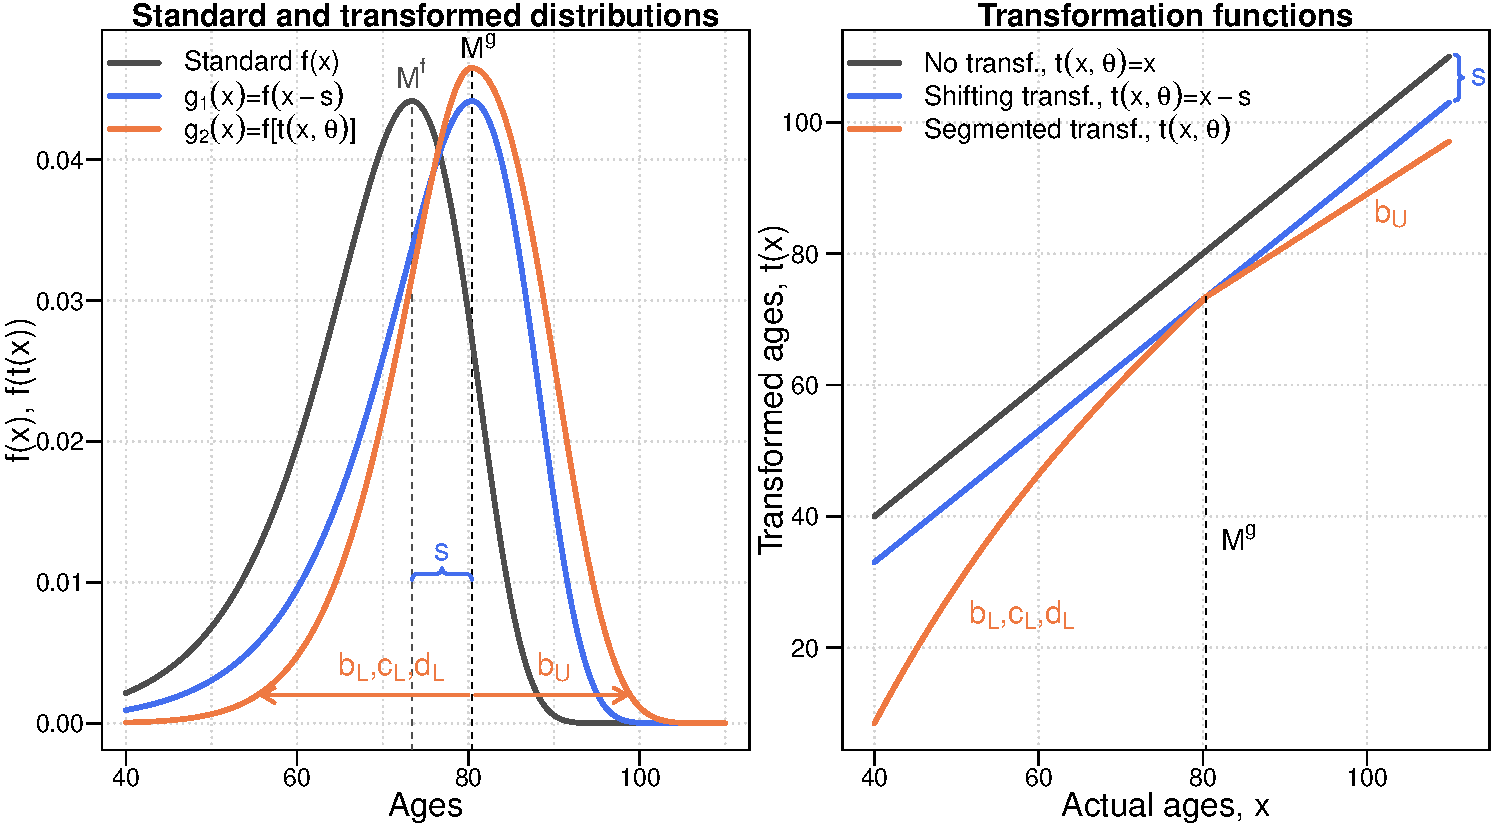
\includegraphics[scale=0.57]{./Figures/F1.pdf} 
		\caption{A schematic overview of the \emph{Cohort Segmented Transformation Age-at-death Distributions} model.\\
		\small \textit{Source}: authors' own elaborations. \label{Fig:CSTADmodel}}    
	\end{center}
\end{figure}

Different parameters' values allow to capture broader mortality developments than the shifting scenario described above. While $b_L$ and $b_U$ modify the variability of the distribution $g_2(x)=f\left[t(x;\bm{\theta})\right]$ (orange line, left panel) w.r.t.~$f(x)$ before and after the modal age at death, $c_L$ and $d_L$ affect the asymmetry and heaviness of the left tail of $g_2(x)$ as compared to $f(x)$. In the example shown in Fig.~\ref{Fig:CSTADmodel}, $b_L > 1$ reduces the variability of $g_2(x)$ before $M^g$ w.r.t.~$f(x)$, while $b_U < 1$ increases the variability of $g_2(x)$ after $M^g$ w.r.t.~$f(x)$. The effects of $c_L$ and $d_L$ are difficult to discern from the left panel. However, the right panel shows the warping transformation $t(x;\bm{\theta})$ applied to $f(x)$ to derive $g_2(x)$; the transformation (orange line) is composed by a cubic function (due to non-zero values of $c_L$ and $d_L$) before the cut-off point $M^g$, and by a linear function above $M^g$.

\subsection{Data}
\label{Subsec:Data}
For illustrative purposes we present outcomes from the proposed model on adult cohort mortality for females in two high-longevity countries, namely Sweden and Denmark. Long-term series of high quality data are available for both countries, even at the very old ages \citep{vaupel1994longer,wilmoth1996extreme,AndreevBookDanemark}, and the two countries display different mortality developments. We therefore test the goodness-of-fit and forecast accuracy of our model with respect to different mortality trajectories \citep{ChristensenEtAlDenmarkSwedenDivergence2010}. The data are derived from the \citeauthor{HMD} (HMD, \citeyear{HMD}), which provides free access to detailed, consistent and high quality historical mortality data for 43 different territories and countries \citep{barbieri2015data}.

Our interest in this article is restricted to the senescent component of mortality, hence we start our analyses from age 40. We therefore cover the age range that is of greater interest for pension and insurance funds. Specifically, we employ two $m \times n$ matrices $\bm{D} = (d_{x,c})$ and $\bm{E} = (e_{x,c})$ containing observed death counts and exposure-to-risk, respectively, classified by age at death $x=40,\ldots, 110+$ and birth cohort $c=1835,\ldots,1970$. Figure~\ref{Fig:Lexis} offers a schematic overview of the data structure by means of two Lexis diagrams: the first (left panel) shows the conventional age-period structure, while the second (right panel) illustrates the age-cohort perspective that we adopt in this paper. On one hand, we select 1835 as starting cohort of analysis for both populations because it is the first cohort with observed data at all ages in Denmark, and to compare the results for the two countries using the same fitting period. On the other hand, 1970 is the final cohort because it contains enough observed data points in both countries (seven in Sweden, six in Denmark) to estimate the three low parameters accurately (cf.~Subsection \ref{Subsec:EstimForeC-STAD}). 

\begin{figure}[t]
	\begin{center}
		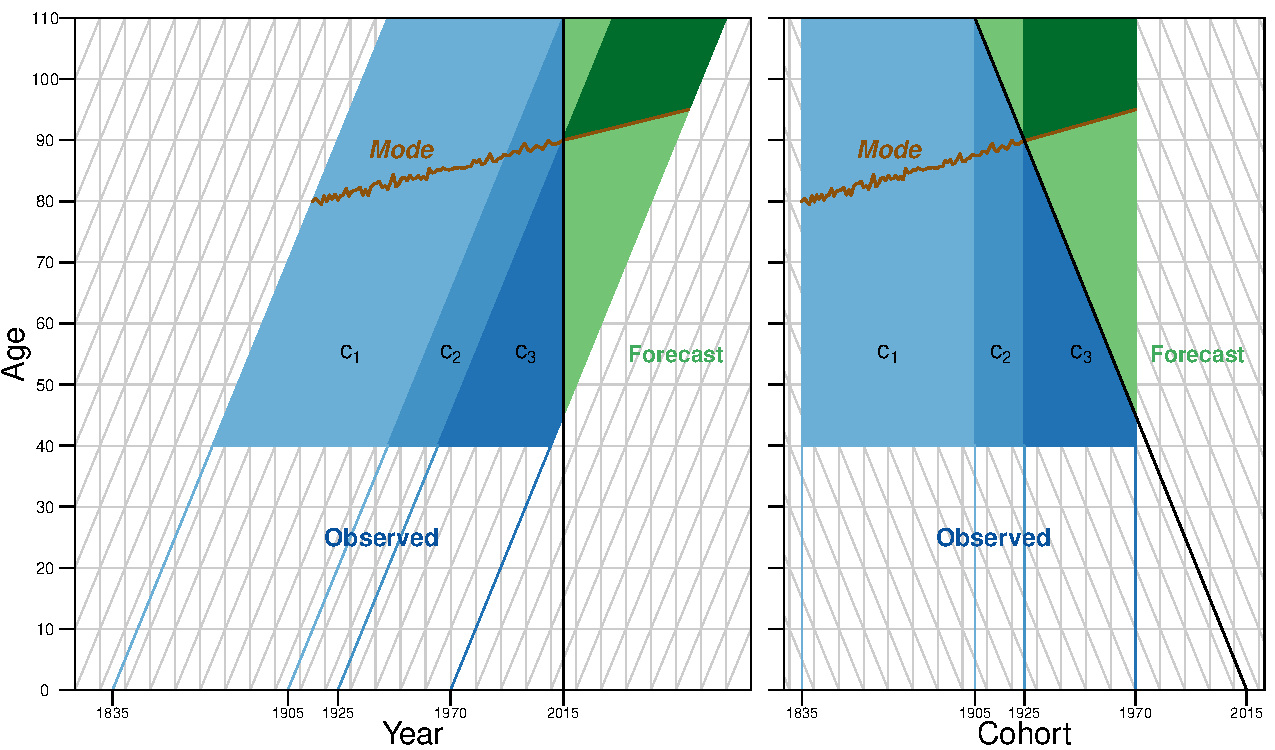
\includegraphics[scale=0.7]{./Figures/F2.pdf} 
		\caption{Conventional age-period (left panel) and age-cohort (right panel) Lexis diagrams illustrating the data structure and the division of cohorts into three groups. Here we assume that: (i) 2015 is the most recent year of data collection, (ii) $\breve{c}=1905$, and (iii) $\tilde{c}=1925$. The three groups are then $c_1=1835, \ldots, 1905$, $c_2=1906, \ldots, 1925$ and $c_3=1926, \ldots, 1970$. The two colours in the forecast years correspond to different parameters' derivations (cf.~Subsection \ref{Subsec:EstimForeC-STAD}): estimation with missing data (light green) and forecasting (dark green). \\
		\small \textit{Source}: authors' own elaborations. \label{Fig:Lexis}}    
	\end{center}
\end{figure}

Estimation and forecasting of the C-STAD parameters (Subsection \ref{Subsec:EstimForeC-STAD}) is performed on three different groups of cohorts. Therefore data are partitioned as follows:
\begin{equation}\label{eq:DataDiv}
\bm{D} = \left[ \bm{D}_{1} : \bm{D}_{2} : \bm{D}_{3}\right] \qquad \bm{E} = \left[ \bm{E}_{1} : \bm{E}_{2} : \bm{E}_{3}\right] \, .
\end{equation}
The first group, denoted by $c_1$, contains the fully observed cohorts $1835,\ldots,\breve{c}$, where $\breve{c}$ corresponds to the last cohort for which all data have been observed. As such, $\bm{D}_{1}$ and $\bm{E}_{1}$ have been observed at all ages $x$ for all cohorts in $c_1$. The second group, denoted by $c_2$, is composed by cohorts $\breve{c}+1, \ldots, \tilde{c}$, where $\tilde{c}$ corresponds to the last cohort for which two age-groups above the adult modal age at death have been observed. In other words, $\bm{D}_{2}$ and $\bm{E}_{2}$ are incomplete, i.e.~data are not available for higher ages and more recent cohorts. However this group of cohorts is selected such that associated $d_{x,c}$ and $e_{x,c}$ have been observed for at least two data points above the modal age $x=M$ for all cohorts in $c_2$. The choice of having two age groups above $M$ is imposed by the estimation of the parameter above the mode (cf.~Subsection~\ref{Subsec:EstimForeC-STAD}). Finally, the third group $c_3$ is composed by the remaining cohorts $\tilde{c}+1, \ldots, 1970$, in which data are only partially available and modal age at death is not observed. An illustration of the divisions of cohorts into the three groups is provided in Figure~\ref{Fig:Lexis}. Figure \ref{Fig:DxExample} shows an example of the observed and missing data for three age-at-death distributions belonging to the different groups of cohorts. 

\begin{figure}[t]
	\begin{center}
		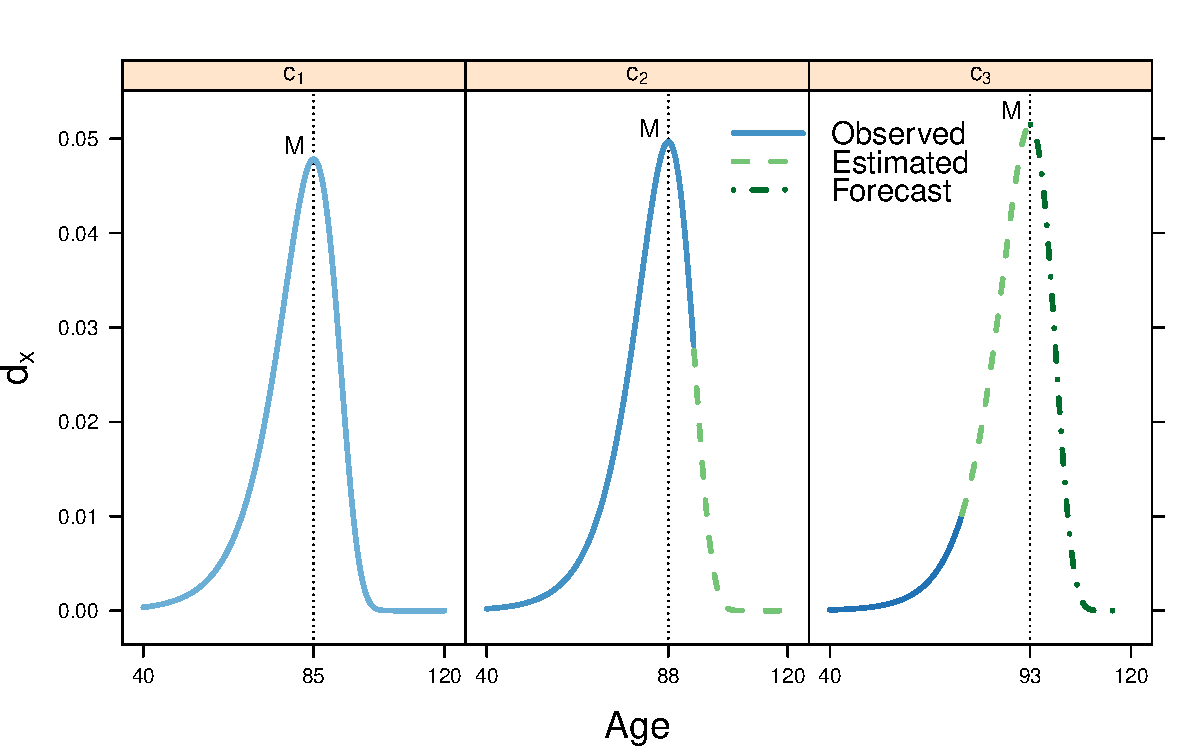
\includegraphics[scale=0.7]{./Figures/F3.pdf} 
		\caption{Example of observed, estimated and forecast data for three age-at-death distributions belonging to the groups of cohorts $c_1$, $c_2$ and $c_3$.\\
		\small \textit{Source}: authors' own elaborations.\label{Fig:DxExample} }    
	\end{center}
\end{figure}

\subsection{The standard distribution}
\label{Subsec:Standard}
The first step in the estimation of the C-STAD model is the derivation of the standard distribution $f(x)$. The C-STAD can be interpreted as a relational model \citep{brass1971scale}, hence it is desirable to include the representative features of the observed data for all cohorts in the computation of $f(x)$. Meanwhile, we also wish to remove the small random fluctuations that characterize the mortality pattern of age-at-death distributions. To achieve both goals at the same time, we derive the age-at-death distribution for each cohort 1835--1970 by a two-dimensional (2D) $P$-splines smoothing approach of cohort mortality \citep{eilers1996flexible, currie2004smoothing}. Specifically, we assume that observed death counts $d_{x,c}$ at given age $x$ and cohort $c$ are realizations of the random variable $D_{x,c}$ which follows a Poisson distribution \citep{brillinger1986biometrics}:
%
\begin{equation}\label{Eq:Poisson}
D_{x,c} \sim \mathcal{P}(e_{x,c} \; \mu_{x,c}) \, ,
\end{equation}
%
where exposure-to-risk $e_{x,c}$ are given and $\mu_{x,c}$ denotes the hazard or force of mortality \cite[such as in, for example,][]{brouhns2002poisson}. We smooth observed death counts using a tensor product of $B$-splines bases over ages and cohorts, and exposures as an offset. To account for uncompleted cohorts and still preserve the rectangular structure in the data, we include regression weights $\bm{W} = (w_{x,c})$ whose elements are equal to one if the corresponding death counts $d_{x,c}$ and exposures $e_{x,c}$ have been observed, and zero otherwise. Smoothing parameters over ages and cohorts are chosen by Bayesian Information Criterion minimization. The \texttt{R} package \texttt{MortalitySmooth} \citep{camarda2012mortalitysmooth} provides a direct implementation of this procedure. 

The estimated smooth mortality surface allows us to derive smooth (partial) densities. We align each density to the distribution of the first cohort (1835), and derive $f(x)$ as the mean of the aligned distributions. This landmark registration procedure has been suggested elsewhere as it enhances the representativeness of $f(x)$ while improving the goodness-of fit of the model \cite[for additional details, see][]{basellini2019modelling}. Importantly, it should be noted that for cohorts in $c_2$ and $c_3$, we only use the part of the aligned distribution corresponding 
to the observed data (i.e.~where regression weights are not zero). 

Finally, we smooth the aligned mean and express the standard density $f(x)$ as a linear combination of equally spaced $B$-spline basis $\bm{B}(x)$ over ages $x$ and coefficients $\bm{\beta}_{f}$ specific to the standard:
%
\begin{equation}\label{Eq:standPsplines}
f(x) = \exp\left[ \bm{B}(x) \, \bm{\beta}_{f} \right] \, .
\end{equation}
In this last step, we chose a generous number of $B$-splines without any penalty term. This whole procedure allows us to preserve all important features in the standard distribution (embodied in $\bm{\beta}_{f}$) after having removed unnecessary random fluctuations from the original data.


\subsection{Estimation and forecast of the C-STAD parameters}
\label{Subsec:EstimForeC-STAD}
Given the estimated standard distribution, we can derive the C-STAD parameters $\bm{\theta}'=\left[s,b_{L},c_{L},d_{L},b_{U}\right]$ for each cohort in 1835--1970. As anticipated in Subsection \ref{Subsec:Data}, we use three different approaches to estimate $\bm{\theta}$, depending on the data available for each cohort; we thus divide cohorts into three groups, as shown in Figure \ref{Fig:Lexis}. 

For the first group of fully observed cohort $c_1$, we start by estimating the parameters vector $\bm{s}$. To properly capture cohort-specific mortality fluctuations, we employ a one-dimensional $P$-spline approach, i.e.~we smooth mortality for each cohort independently, numerically compute the corresponding density and extract the modal ages at death for each cohort \citep[for a similar approach in a period perspective, see][]{ouellette2011changes}. From the modal ages we estimate the parameter $\hat{\bm{s}}=\left(\hat{s}_{c}=M_{c} - M_f\right)$ over cohorts in $c_1$, where $M_f$ denotes the mode of the standard distribution, which by construction corresponds to the modal age at death for the cohort born in 1835. \par

Having derived an estimate of the shifting parameter $\hat{\bm{s}}$, we can estimate the remaining parameters $\bm{\alpha}'=\left[b_{L},c_{L},d_{L},b_{U}\right]$. We take advantage of the Poisson assumption in Eq.~(\ref{Eq:Poisson}) and maximise the following log-likelihood function:
%
\begin{equation}\label{Eq:loglikeC1}
\ln\mathcal{L}_{\bm{\alpha}}\left(\bm{\alpha}\,|\,d_{x,c} , e_{x,c} , w_{x,c} , \hat{s}_{c}, \bm{\beta}_{f}
\right) \propto \sum_{x} w_{x,c} \left[  d_{x,c} \,
\ln \left( \mu^{\texttt{C-STAD}}_{x,c}  \right) - e_{x,c}
\, \mu^{\texttt{C-STAD}}_{x,c} \right] 
\end{equation}
%
for each cohort $c = 1835,\ldots,\breve{c}$, where regression weights $w_{x,c}$ are zero in the case of unobserved data at the highest ages, and $\mu^{\texttt{C-STAD}}_{x,c}$ denotes the estimated hazard of the C-STAD model. In words, the optimization procedure looks for a combination of parameters $\hat{\bm{\alpha}}$ that produces, for each cohort, an age-at-death distribution whose corresponding hazard maximises the log-likelihood in Eq.~(\ref{Eq:loglikeC1}). The associated age-at-death distribution can be written as follows:
\begin{equation}\label{eq:gBspl}
\hat{g}_{c}(x) = \exp\left[ B(x_{t}) \bm{\beta}_{f} \right] \qquad \mbox{where} \quad x_{t} = t(x; \hat{s}_{c},\hat{\bm{\alpha}}) \, .
\end{equation}
The hazard corresponding to $\hat{g}_{c}(x)$ is computed using standard life-table formulas \citep{preston2001demogr}.

For the second group of partially observed cohorts $c_2$, we start again from the shifting parameter $\bm{s}$. We use the same estimation approach used in $c_1$: data are available until the ages above the mode, therefore the smoothing approach produces an estimate of $M_c$ and $\hat{\bm{s}}$ over cohorts in $c_2$. With respect to the remaining parameters, we also follow the same approach: we maximize Eq.~\eqref{Eq:loglikeC1} for each cohort $c=\breve{c}+1,\ldots,\tilde{c}$, the only difference being that zero regression weights correspond to the missing data above the mode of the partially observed cohorts. It should be noted here that the missing data only influence the estimation of $b_U$, as complete data are observed below the mode for all cohorts in this group. 

For the third group of partially observed cohorts $c_3$, we employ a mixture of forecasting and estimation to determine the C-STAD parameters. The lack of data above the modal age at death makes it impossible to estimate the parameter $\bm{s}$ and compute the log-likelihood in Eq.~\eqref{Eq:loglikeC1}. Hence, we start from the time-series of the estimated parameters $\hat{\bm{s}}$ and $\hat{\bm{b}}_U$ over cohorts in $c_1$ and $c_2$ to compute their forecasts for cohorts $c_3$. 

From a theoretical perspective, these two parameters are related by the fact that only mortality changes occurring above the mode can modify its value \cite[cf.~Appendix B in][]{canudas2010three}. Correlation analyses for the two countries under study confirm the strong relation between the two series (Pearson correlation of 0.96 and 0.90 for the time-series in first differences for Sweden and Denmark, respectively). As such, we specify a vector autoregressive (VAR) model of order one with constant for the two (differenced) parameters, and we forecast their values for all cohorts $c_3$. The \texttt{R} package \texttt{vars} allows us to perform model selection and estimation \citep{pfaff2008analysis,pfaff2008var}.

Then, we take the forecast values of $\hat{\bm{s}}$ and $\hat{\bm{b}}_U$ as given, and we estimate the remaining parameters $\breve{\bm{\alpha}}'=\left[b_{L},c_{L},d_{L}\right]$ by maximizing the log-likelihood:
%
\begin{equation}\label{Eq:loglikeC3}
%\begin{aligned}
\ln\mathcal{L}_{\breve{\bm{\alpha}}}\left(\breve{\bm{\alpha}}\,|\,d_{x,c} , e_{x,c} , w_{x,c} , \hat{s}_{c}, \hat{b}_{U_{c}} , \bm{\beta}_{f} \right) \propto  \sum_{x} w_{x,c} \, \left[  d_{x,c} \,
\ln \left( \mu^{\texttt{C-STAD}}_{x,c}  \right) - e_{x,c}
\, \mu^{\texttt{C-STAD}}_{x,c} \right] 
%\end{aligned}
\end{equation}
%
for each cohort $c=\tilde{c}+1,\ldots,1970$. In contrast to the estimation procedure in $c_2$, here the missing data influence the estimation of the parameters associated to the ages below the modal age at death. \par

The estimate $\hat{\bm{\theta}}$ for each cohort in 1835--1970 allows us to derive a complete set of age-specific mortality measures, i.e.~we can complete the mortality experience for the partially observed cohorts of our analysis. In order to derive the C-STAD confidence intervals (CI)\footnote{to avoid confusion, we use the general term CI for all cohorts analysed, even when intervals are constructed from the mixture of forecast and estimated parameters (i.e.~cohorts $c_3$).}, we employ a bootstrapping procedure \citep{efron1994introduction}. As suggested by \cite{keilman2006prediction}, we consider the uncertainty related to: (i) the estimated parameters, and (ii) the forecast values of $\bm{s}$ and $\bm{b}_U$. The first source of uncertainty is accounted for by generating bootstrap death counts from the C-STAD deviance residuals \cite[as in, for example,][]{koissi2006evaluating,renshaw2008simulation,ouellette2012regional}. Appendix \ref{Appendix:ResidualDeath} provides more details on the computation of deviance residuals and bootstrap death counts. The second source of uncertainty is considered by simulating future values of the VAR model. We employ 40 different matrices of bootstrap death counts, and for each of these, we refit the C-STAD model and simulate 40 future values of $\bm{s}$ and $\bm{b}_U$. From the 1600 resulting simulations, we take the lower and higher deciles to construct 80\% pointwise confidence intervals.

Finally, routines developed to fit and forecast the C-STAD model were implemented in \texttt{R} \citep{Rcite} and are publicly available, and all the results presented in the following Section are fully reproducible at \url{https://github.com/ubasellini/C-STAD}. 

\section{Results}
\label{Sec:Results}

\subsection{Out-of-sample validation of the C-STAD model}
\label{Subsec:Out-of-sample}
Before estimating the proposed C-STAD model to complete partially observed cohorts, we first assess the accuracy of the C-STAD model by performing six predictive out-of-sample validation exercises on Swedish and Danish adult females. Specifically, we pretend that the last year of collected data is $2015 - \delta$, where $\delta=10,15,20,25,30$ and 35 years. We then fit the C-STAD model to the fully observed cohorts $c_1=1835,\ldots,1905-\delta$ and we forecast mortality $\delta$ years ahead. We then compare the forecast life expectancy at age 40 ($e_{40}$) and the Gini coefficient at age 40 ($g_{40}$)\footnote{in all analyses, we multiplied the Gini value by 100 in order to have a comparable magnitude with $e_{40}$.} with the observed out-of-sample values. Both measures of longevity (the former) and lifespan variability (the latter, which further measures the lifespan inequality within a population) are indeed useful to evaluate the accuracy of mortality forecasts \citep{bohk2017lifespan}.

An explicative example of this procedure is useful to clarify the out-of-sample exercises. Let us consider $\delta=10$: then, the last year of fully observed data is 2005. We fit the C-STAD to the fully observed cohorts $c_1=1835,\ldots,1895$, and we forecast 10-year ahead. By doing so, we complete the mortality experience of the partially observed cohorts $1896,\ldots,1905$, and for each of these, we compute and compare the estimated $e_{40}$ and $g_{40}$ with the observed ones. 

It is worth mentioning at this point that, for the lower values of $\delta$, forecasting is achieved simply by fitting the C-STAD on the partially observed cohorts $c_2$. In the explicative example above, where the last data collection occurred in 2005, the cohort 1896, for instance, has been observed at all ages except 110. We thus take advantage of the nature of cohort data and consider all possible observations to complete the mortality experience of this partial cohort.  Conversely, for higher values of $\delta$, forecasting is achieved by considering also the cohorts $c_3$, which require the combination of forecasting and estimation of the C-STAD parameters. 

In addition to the C-STAD, we perform the same out-of-sample exercises with the 2D $P$-splines approach of \cite{currie2004smoothing}. This is indeed the only model that, up to our knowledge, has been employed to forecast cohort mortality from a cohort perspective \citep{cmi2007stochastic} and is readily implemented in the \texttt{R} software \cite[in the \texttt{MortalitySmooth} package,][]{camarda2012mortalitysmooth}. We do not consider other methodologies, such as the \cite{lee1992modeling} model and its variants, because cohort forecasts with these approaches are derived from period ones, and the comparison would not be objective (for example, forecast values depend on the length of the fitting period, whose choice would be subjective and not comparable in such exercise).  

Table \ref{Table:RMSE} presents the results of our analysis. The first and second columns contain the cohorts used for fitting and forecasting the C-STAD and 2D $P$-splines models, respectively. The third column contains the forecast horizon of the out-of-sample exercise, while the fourth column the measure analysed ($e_{40}$ and $g_{40}$). Results are shown in the last four columns. We assess the accuracy of the point forecasts by computing the root mean square error (RMSE):
%
\begin{equation}\label{Eq:RMSE}
\mathrm{RMSE}=\sqrt{\frac{1}{\delta} \sum_{c=1}^{\delta} \left(\hat{y}_c-y_c\right)^2} \, , \notag
\end{equation} 
%
where $\delta$ is the forecasting horizon, and $\hat{y}_c$ and $y_c$ are the forecast and observed out-of-sample values of either $e_{40}$ or $g_{40}$. 

% TABLE RMSE: 10, 20, 30 YEARS
\begin{table}[h!]
	\small
	\centering
	\begin{tabular}{cccccc|cc}
		\toprule
		& & & &   \multicolumn{2}{c}{\textbf{Sweden}}    & \multicolumn{2}{c}{\textbf{Denmark}} \\
		
		\cmidrule{5-8}	
		
		\thead{Fitting \\ cohorts}  & \thead{Forecast \\ cohorts} & Horizon &  Measure  &  C-STAD   & 2D $P$-spline &  C-STAD   & 2D $P$-spline     \\ 
		\midrule	
		%%%% FIRST EXERCISE	
		\rowcolor{my-white} 
		\multicolumn{1}{c}{\cellcolor{my-white}}   &
		\multicolumn{1}{c}{\cellcolor{my-white}}   & \multicolumn{1}{c}{\cellcolor{my-white}}               & \multicolumn{1}{c|}{\cellcolor{my-white}$e_{40}$} & 0.08  & \textbf{0.08} &  \textbf{0.08} &  0.08      \\
		\rowcolor{my-white} 
		\multicolumn{1}{c}{\multirow{-2}{*}{\cellcolor{my-white}1835--1895}}  &  \multicolumn{1}{c}{\multirow{-2}{*}{\cellcolor{my-white}1896--1905}}  & 
		\multicolumn{1}{c}{\multirow{-2}{*}{\cellcolor{my-white}10y}}& \multicolumn{1}{c|}{\cellcolor{my-white}$g_{40}$} & \textbf{0.09} &   0.10 & \textbf{0.08} &  0.08  \\
		
		%%%% SECOND EXERCISE	
		\hhline{|--------|}
		\rowcolor{my-grey} 
		\multicolumn{1}{c}{\cellcolor{my-grey}}  & \multicolumn{1}{c}{\cellcolor{my-grey}}             &
		\multicolumn{1}{c}{\cellcolor{my-grey}}  & \multicolumn{1}{c|}{\cellcolor{my-grey}$e_{40}$} & \textbf{0.07} &  0.09 & \textbf{0.07} & 0.08  \\
		\rowcolor{my-grey}       \multicolumn{1}{c}{\multirow{-2}{*}{\cellcolor{my-grey}1835--1890}} &      \multicolumn{1}{c}{\multirow{-2}{*}{\cellcolor{my-grey}1891--1905}}               &
		\multicolumn{1}{c}{\multirow{-2}{*}{\cellcolor{my-grey}15y}}               & \multicolumn{1}{c|}{\cellcolor{my-grey}$g_{40}$} & \textbf{0.08} &  0.10 & \textbf{0.07} & 0.12       \\ 
		
		%%%% THIRD EXERCISE
		\hhline{|--------|}
		\rowcolor{my-white} 
		\multicolumn{1}{c}{\cellcolor{my-white}}   &
		\multicolumn{1}{c}{\cellcolor{my-white}}   &    \multicolumn{1}{c}{\cellcolor{my-white}}                & \multicolumn{1}{c|}{\cellcolor{my-white}$e_{40}$} &  \textbf{0.05} & 0.08 & \textbf{0.06} & 0.08 \\
		\rowcolor{my-white}            
		\multicolumn{1}{c}{\multirow{-2}{*}{\cellcolor{my-white}1835--1885}}           &
		\multicolumn{1}{c}{\multirow{-2}{*}{\cellcolor{my-white}1886--1905}}               &
		\multicolumn{1}{c}{\multirow{-2}{*}{\cellcolor{my-white}20y}}               & \multicolumn{1}{c|}{\cellcolor{my-white}$g_{40}$} & \textbf{0.09} & 0.11 & \textbf{0.06} & 0.12  \\
		
		%%%% FOURTH EXERCISE	
		\hhline{|--------|}
		\rowcolor{my-grey} 
		\multicolumn{1}{c}{\cellcolor{my-grey}}   &
		\multicolumn{1}{c}{\cellcolor{my-grey}}   & \multicolumn{1}{c}{\cellcolor{my-grey}}               & \multicolumn{1}{c|}{\cellcolor{my-grey}$e_{40}$} & \textbf{0.04} & 0.08  & \textbf{0.03} &  0.08     \\
		\rowcolor{my-grey} 
		\multicolumn{1}{c}{\multirow{-2}{*}{\cellcolor{my-grey}1835--1880}}                 &  \multicolumn{1}{c}{\multirow{-2}{*}{\cellcolor{my-grey}1881--1905}}  & 
		\multicolumn{1}{c}{\multirow{-2}{*}{\cellcolor{my-grey}25y}}  & \multicolumn{1}{c|}{\cellcolor{my-grey}$g_{40}$} & \textbf{0.10} & 0.11 & \textbf{0.11} & 0.14      \\
		
		%%%% FIFTH EXERCISE
		\hhline{|--------|}
		\rowcolor{my-white} 
		\multicolumn{1}{c}{\cellcolor{my-white}}             &
		\multicolumn{1}{c}{\cellcolor{my-white}}             & \multicolumn{1}{c}{\cellcolor{my-white}}             & \multicolumn{1}{c|}{\cellcolor{my-white}$e_{40}$} &   \textbf{0.06} & 0.09 &  \textbf{0.03} &  0.11   \\
		\rowcolor{my-white} 
		\multicolumn{1}{c}{\multirow{-2}{*}{\cellcolor{my-white}1835--1875}} &      \multicolumn{1}{c}{\multirow{-2}{*}{\cellcolor{my-white}1876--1905}}               &
		\multicolumn{1}{c}{\multirow{-2}{*}{\cellcolor{my-white}30y}}               & \multicolumn{1}{c|}{\cellcolor{my-white}$g_{40}$} & \textbf{0.10} &  0.14 & \textbf{0.11} & 0.19       \\
		
		%%%% SIXTH EXERCISE
		\hhline{|--------|}
		\rowcolor{my-grey} 
		\multicolumn{1}{c}{\cellcolor{my-grey}}   &   
		\multicolumn{1}{c}{\cellcolor{my-grey}}   &  \multicolumn{1}{c}{\cellcolor{my-grey}}                & \multicolumn{1}{c|}{\cellcolor{my-grey}$e_{40}$} & 0.14 & \textbf{0.08} & \textbf{0.05} &  0.14  \\
		\rowcolor{my-grey}           
		\multicolumn{1}{c}{\multirow{-2}{*}{\cellcolor{my-grey}1835--1870}}           &
		\multicolumn{1}{c}{\multirow{-2}{*}{\cellcolor{my-grey}1871--1905}}               &
		\multicolumn{1}{c}{\multirow{-2}{*}{\cellcolor{my-grey}35y}}               & \multicolumn{1}{c|}{\cellcolor{my-grey}$g_{40}$} & \textbf{0.04} &  0.13 & \textbf{0.06} & 0.22   \\		
		
		\bottomrule 
		
	\end{tabular}
	\caption{Root mean square error (RMSE) of the C-STAD and 2D $P$-spline forecasts of $e_{40}$ and $g_{40}$ for adult females in Sweden and Denmark in six out-of-sample validation exercises: forecast horizon of 10, 15, 20, 25, 30 and 35 years. Lower values of the RMSE (in bold, assessed using all available decimals) correspond to greater forecast accuracy.\\
	\small \textit{Source}: authors' elaborations on data from the \cite{HMD}.}\label{Table:RMSE}
\end{table}

The table shows that the C-STAD forecasts are accurate in completing the mortality experience of partially observed cohorts. The RMSE values of both $e_{40}$ and $g_{40}$  are low across the six exercises, and they do not increase significantly with the forecasting horizon. Additionally, C-STAD forecasts are more accurate than those of the 2D $P$-spline model. Very similar results are obtained by employing different prediction accuracy measures, such as the MAPE and MAE (see Appendix \ref{Appendix:AdditResults}). \par

\subsection{Mortality developments for Swedish and Danish females, cohorts 1835--1970}
\label{Subsec:ForecastC-STAD}
In this Subsection we show the results of employing the C-STAD model to estimate and forecast adult female cohort mortality in Sweden and Denmark for the cohorts 1835--1970. The estimated and forecast parameters are shown in Appendix \ref{Appendix:AdditResults}. Figure \ref{Fig:CSTADfitE40G40} shows the observed and fitted remaining life expectancies at age 40 ($e_{40}$) and Gini coefficient at age 40 ($g_{40}$) in the two population analysed for the fully observed cohorts $c_1$ (1835--$\breve{c}$, where $\breve{c}$ is 1906 for Sweden and 1905 for Denmark). The two graphs provide evidence on the goodness-of-fit of the C-STAD model, whose estimates are very close to the observed values for both measures in the two populations. Inspection of the deviance residuals (shown in Appendix \ref{Appendix:AdditResults}) provides additional evidence on the adequacy of the C-STAD model. \par

\begin{figure}[t]
	\begin{center}
		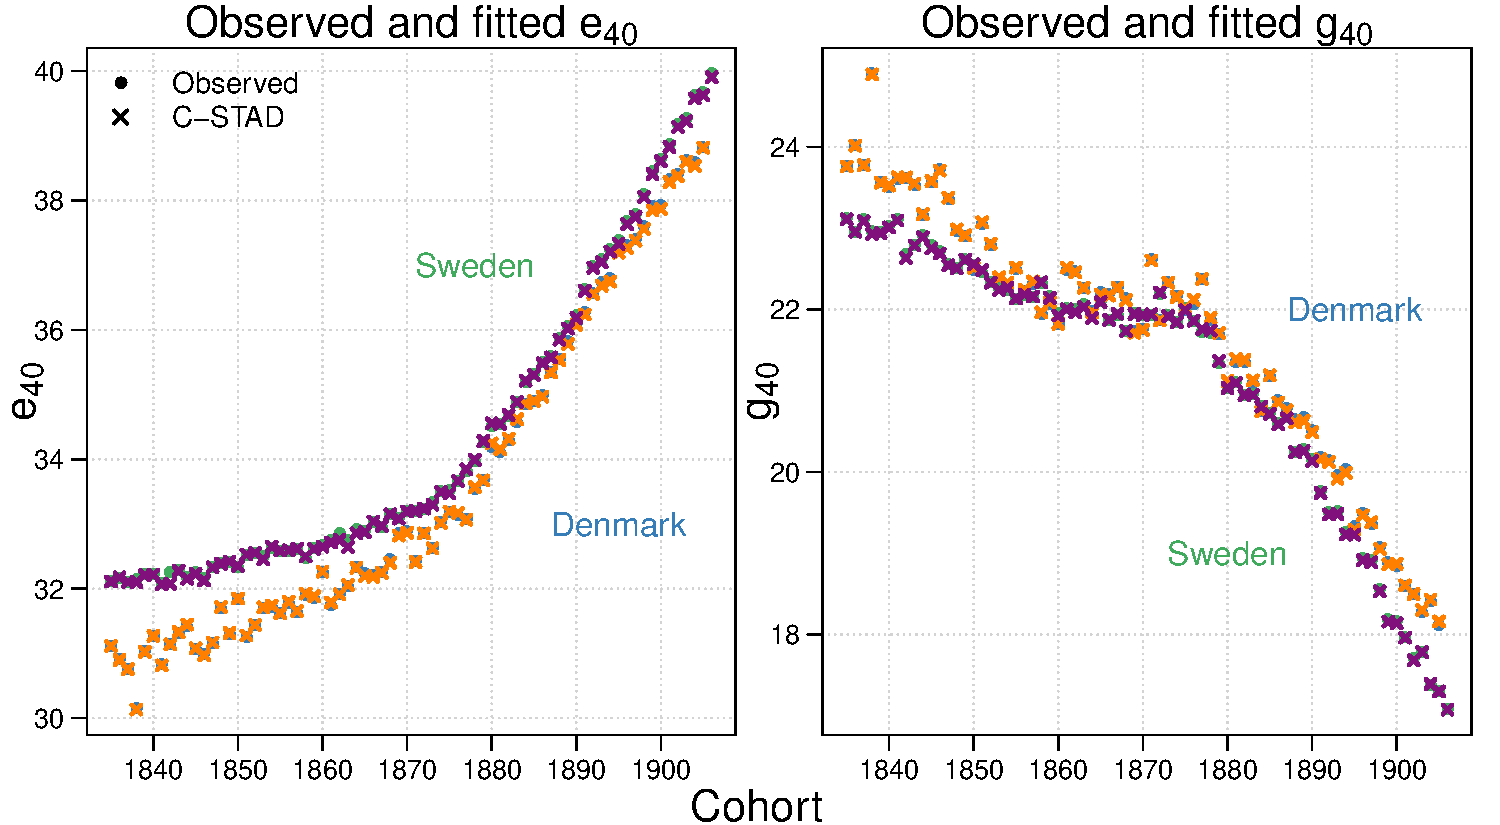
\includegraphics[scale=0.57]{./Figures/F4.pdf} 
		\caption{Observed and C-STAD estimated remaining life expectancies at age 40 ($e_{40}$, left panel) and Gini coefficient at age 40 ($g_{40}$, right panel) for adult females in Sweden and Denmark for the fully observed cohorts 1835--$\breve{c}$ (where $\breve{c}$ is 1906 for Sweden and 1905 for Denmark).\\ \small \textit{Source}: authors' elaborations on data from the \cite{HMD}.\label{Fig:CSTADfitE40G40}}    
	\end{center}
\end{figure}

Figure \ref{Fig:CSTADforeE40G40} shows the observed (cohorts $c_1$) and completed ($c_2$ and $c_3$) $e_{40}$ and $g_{40}$ computed with the C-STAD (with 80\% pointwise confidence intervals) and 2D $P$-spline model for the two population analysed. Despite sharing similar country trends in the fully observed cohorts $c_1$, it is interesting to observe the different mortality developments in the partially observed cohorts $c_2$: while Swedish adult females show continuous improvements in longevity and lifespan equality, Danish ones display a stagnation of $e_{40}$ and an increase in lifespan inequality. The trends of the mortality measures for the partially observed cohorts are similar across the models, with the exception of Danish $e_{40}$: the increase of the 2D $P$-spline forecast $e_{40}$ is much faster then for the C-STAD model, resulting in a crossover among the two populations. Moreover, it is interesting to observe that the C-STAD confidence intervals are rather narrow for both countries in $c_2$ (as the great majority of data is observed for these cohorts), while they increase in the cohorts $c_3$ proportionally to the amount of missing data. Note that $\tilde{c}$ is 1925 and 1927 for Sweden and Denmark, respectively.  

\begin{figure}[t]
	\begin{center}
		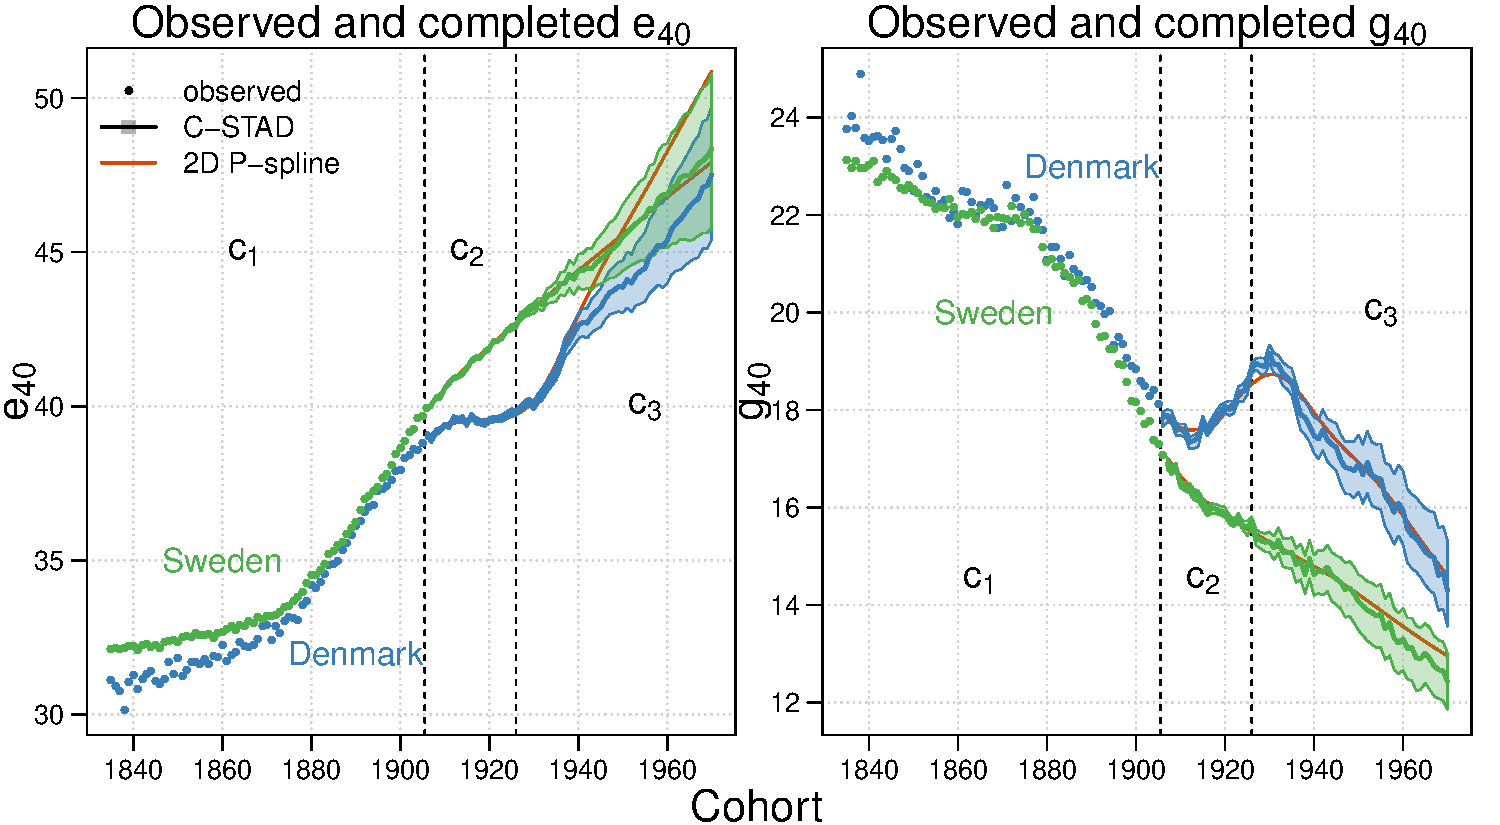
\includegraphics[scale=0.57]{./Figures/F5.pdf} 
		\caption{Observed (cohorts $c_1$) and completed ($c_2$ and $c_3$) remaining life expectancies at age 40 ($e_{40}$, left panel) and Gini coefficient at age 40 ($g_{40}$, right panel) for the C-STAD (with 80\% confidence intervals) and 2D $P$-spline models for adult females in Sweden and Denmark for the cohorts 1835--1970.\\ \small \textit{Source}: authors' elaborations on data from the \cite{HMD}.\label{Fig:CSTADforeE40G40}}    
	\end{center}
\end{figure}

The age-specific mortality rates analysis shown in Figure \ref{Fig:CSTADforeMx} offers additional insights on cohort mortality developments of the two populations. In the top panels, observed, fitted and forecast mortality rates over cohorts are shown for some selected ages. In addition to the goodness-of-fit of the C-STAD model, the graphs highlight diverse age-specific developments in the two countries: for example, mortality at ages 40 and 60 of Danish cohorts born at the beginning of the twentieth century did not improve, resulting in the atypical trends of the summary measures shown in Figure \ref{Fig:CSTADforeE40G40} (stagnation of $e_{40}$ and increase of $g_{40}$). In the bottom panels, mortality rates over all ages are shown for some selected cohorts. This second perspective shows how the shape of the mortality curve, appropriately captured by the C-STAD model, changed over time: for example, mortality at young adult ages was still relatively high in both countries for the 1835 cohort, with the curve being rather flat in the age range 40--50. The subsequent mortality decline at all ages, mainly attributable to improvements in sanitary environment, public hygiene and nutrition \citep{mckeown1976modern}, clearly emerges from Figure \ref{Fig:CSTADforeMx}. An additional interesting observation is that the confidence intervals of the C-STAD widens as expected: for example, variability increases with age for the completed cohorts, as fewer age-specific data have been observed at higher ages. Finally, Figure \ref{Fig:CSTADforeDx} shows the observed and C-STAD age-at-death distributions for the three cohorts analysed in the previous panels. 

\begin{figure}[h!]
	\begin{center}
		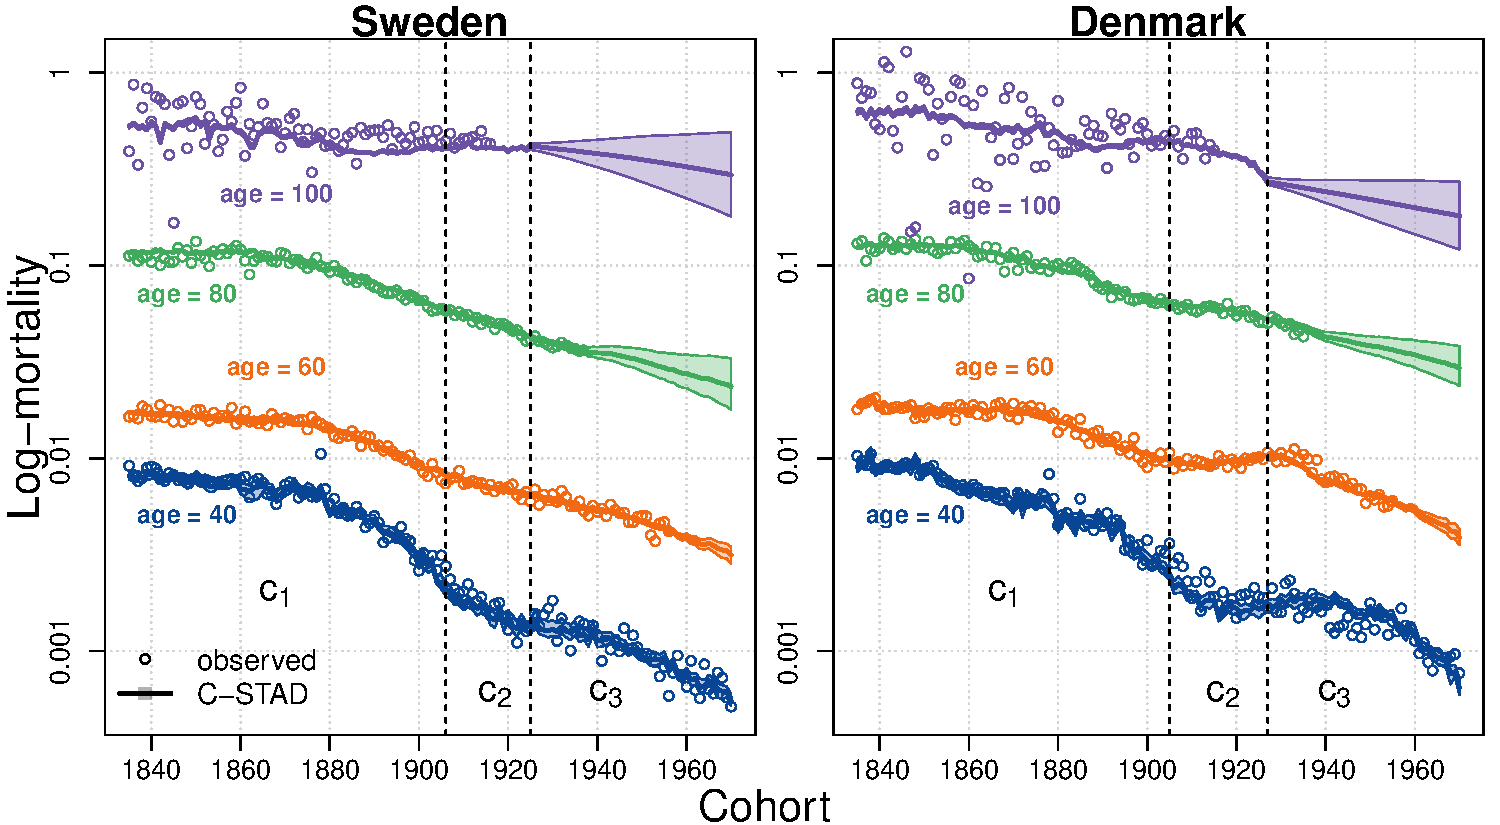
\includegraphics[scale=0.57]{./Figures/F6a.pdf} 
		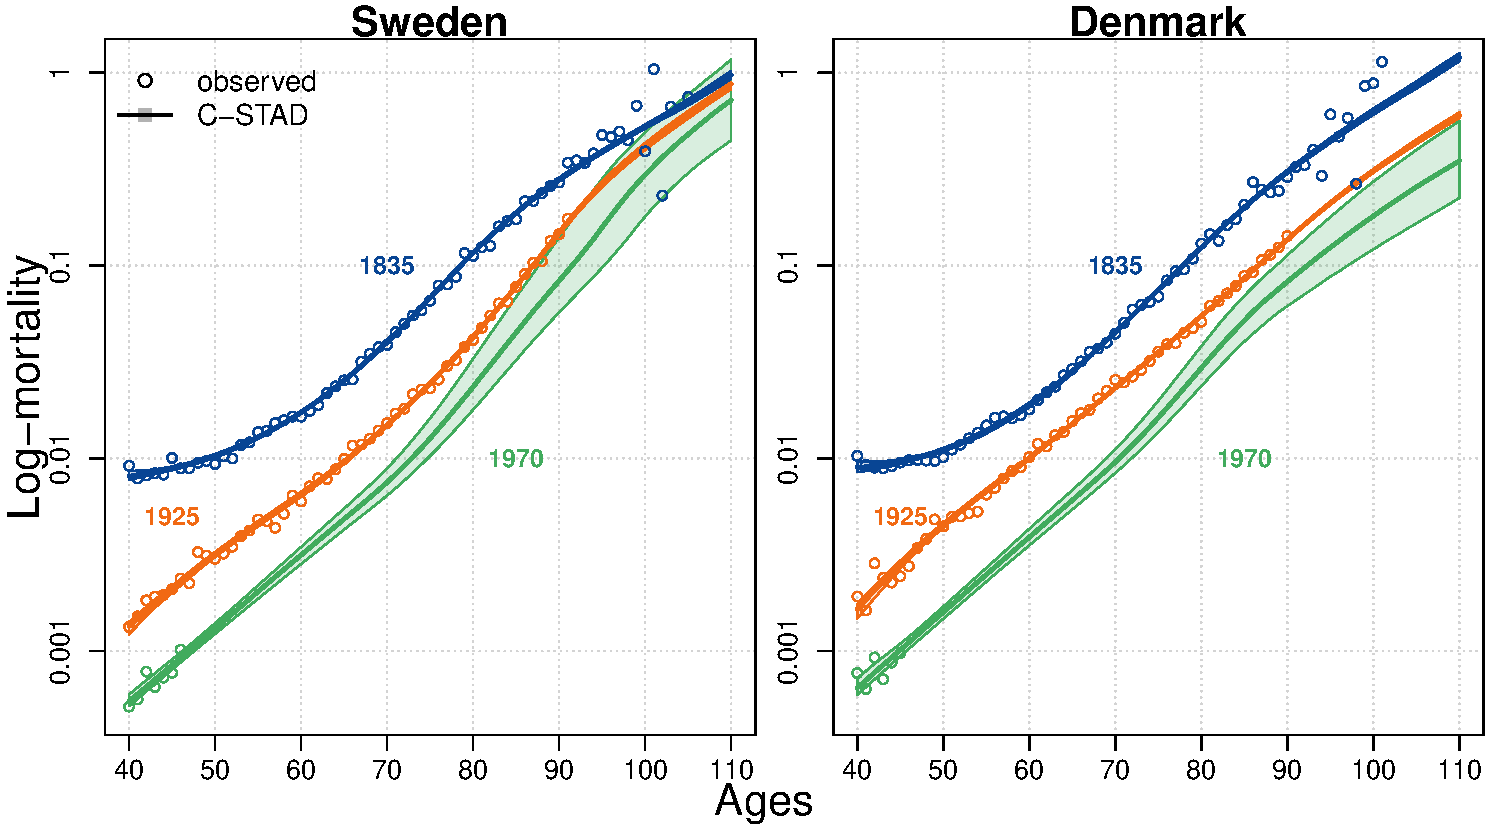
\includegraphics[scale=0.57]{./Figures/F6b.pdf} 
		\caption{Observed, fitted and forecast age-specific mortality rates for selected ages (top panels) and for selected cohorts (bottom panels) with 80\% confidence intervals for females in Sweden and Denmark aged 40-110+ for the cohorts 1835--1970.\\ \small \textit{Source}: authors' elaborations on data from the \cite{HMD}.\label{Fig:CSTADforeMx}}    
	\end{center}
\end{figure}

\begin{figure}[h!]
	\begin{center}
		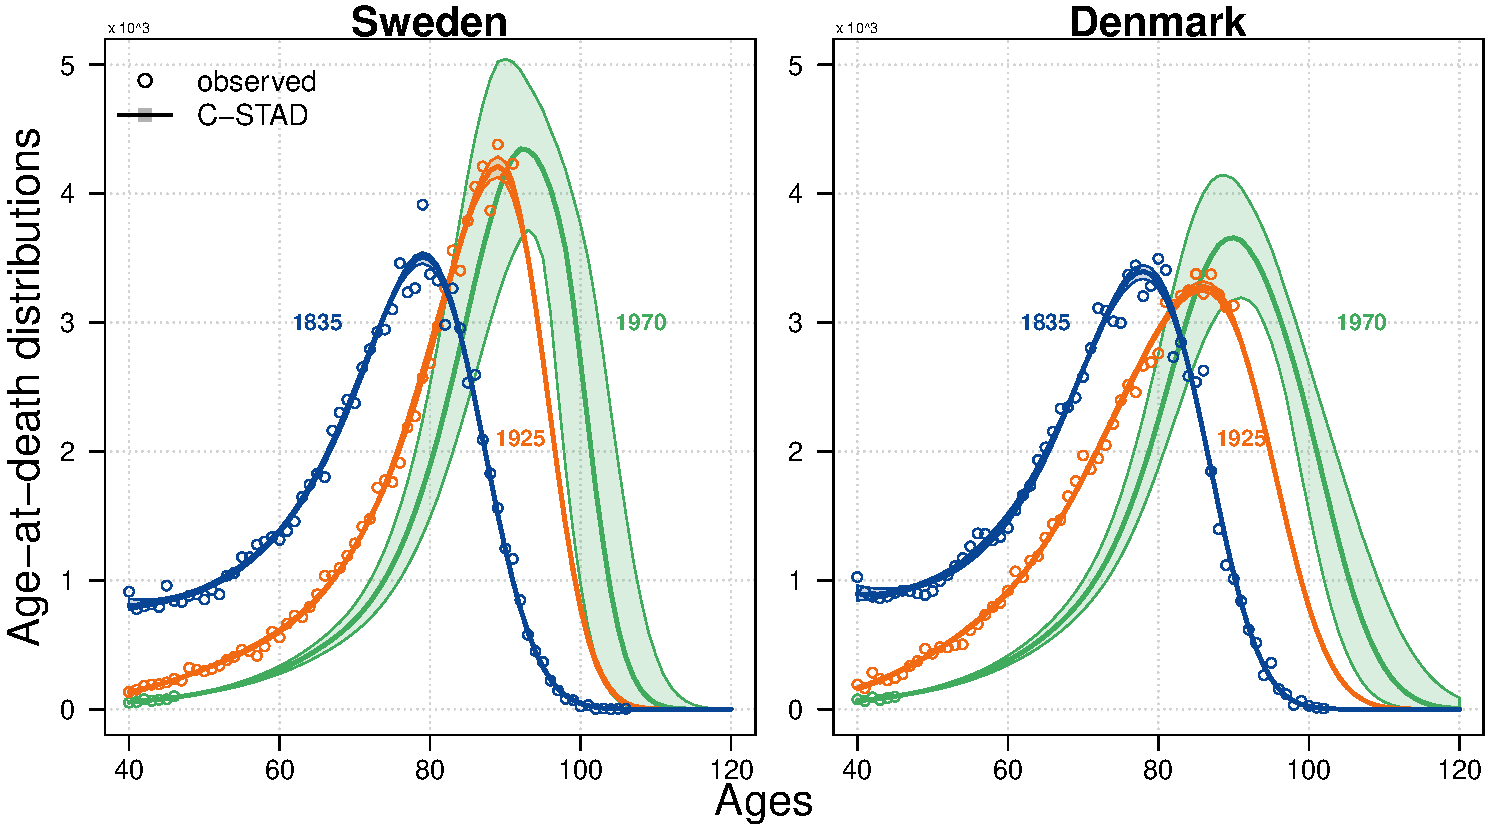
\includegraphics[scale=0.57]{./Figures/F7.pdf}  
		\caption{Observed, fitted and forecast age-at-death distributions for selected cohorts (bottom panels) with 80\% confidence intervals for females in Sweden and Denmark aged 40-110+.\\ \small \textit{Source}: authors' elaborations on data from the \cite{HMD}.\label{Fig:CSTADforeDx}}    
	\end{center}
\end{figure}

\section{Discussion} 
\label{Sec:Discussion}
Mortality forecasting has drawn considerable interest in recent decades among academics and financial sector practitioners due to the increasing challenges posed by population ageing. Advances in the field have almost exclusively been made on period mortality, as the most recent and innovative techniques are based on modelling and forecasting different functions of period life tables \cite[see, for example,][]{lee1992modeling,cairns2006two,raftery2013bayesian}. When considered, cohort effects in mortality modelling and forecasting are typically analysed within an age-period perspective \citep{renshaw2006cohort,cairns2009quantitative,plat2009stochastic,dokumentov2018bivariate}.  
 
In this article, we take an alternative perspective and introduce a new methodology to model and forecast mortality from cohort data. An important advantage of cohort forecasts is that they allow to complete the mortality experience of non-extinct cohorts, thus enabling the derivation of their mortality developments. Our approach focuses on cohort age-at-death distributions: specifically, we propose a warping transformation of the age-axis of a standard distribution to describe and forecast adult mortality developments across cohorts. Since we focus on the cohort perspective, we denote our methodology \emph{Cohort Segmented Transformation Age-at-death Distributions} (C-STAD) model. Warping transformations and skewing procedures have already been fruitfully employed to model distributional changes \cite[see, e.g.,][]{fernandez1998bayesian,camarda2008warped}. 

Our methodology is inspired by the Segmented Transformation Age-at-death Distributions (STAD) model recently proposed by \cite{basellini2019modelling} to forecast adult age-at-death distributions. In addition to shifting the focus from period to cohort mortality, our methodology extends the STAD to a cubic transformation before the modal age at death. The additional parameters $c_L$ and $d_L$ are indeed necessary to adequately describe cohort mortality developments at young adult ages. A possible explanation for this is related to the significant improvements in mortality, especially at younger adult ages, across the cohorts that we analyse (cf.~Fig.~\ref{Fig:CSTADforeMx}). Non-linear transformation functions above the mode were tested too, but they did not provide a better fit compared to a linear transformation function. 

Only a handful of models have been proposed to directly forecast cohort mortality so far \citep{chiou2009modeling,zanotto2017reconstruction,rizzi2019forecasting}. One of the main reasons for the limited efforts in this direction is the heavy data demands that such models require. However, this problem is reduced when only adult mortality is considered \citep{booth2006demographic}. As such, the issue does not affect us to a great extent, as our interest in this article is restricted to adult mortality only. 

We have shown the results of fitting and forecasting cohort mortality with the C-STAD model for Swedish and Danish adult females for the cohorts 1835--1970. Our methodology is accurate from a point forecast perspective: for each population, we performed six out-of-sample validation exercises of different forecast horizons. The resulting point forecast errors are generally small, even for the longer forecast horizons. Additionally, the C-STAD forecasts are consistently more precise than those of the 2D $P$-spline model of \cite{currie2004smoothing}, which has been already used to directly forecast cohort mortality \citep{cmi2007stochastic}. 

Our results allow us to derive age-specific and summary measures of mortality, such as remaining life expectancy and Gini coefficient at age 40 ($e_{40}$ and $g_{40}$), for all cohorts of the population analysed. Although following similar trends to the 2D $P$-spline model, C-STAD estimates of $e_{40}$ seem more coherent when considered together, lacking the rapid increase and cross-over of Danish forecast displayed by the 2D model. With respect to Danish forecasts, it is interesting to observe a stagnation of $e_{40}$ and an increase of $g_{40}$ for the cohorts 1910--1930. Such results are consistent with other findings in the literature \cite[see, e.g., Fig.~4 in][]{jacobsen2002long}, which have been attributed to the smoking behaviour of Danish women \citep{jacobsen2006causes,lindahl2016did}. 

To conclude, the C-STAD model offers great prospects for mortality forecasting from the cohort perspective. Insurance companies would benefit from employing our model to assess their solvency needs, as the model provides a direct approach to complete the mortality experience  of non-extinct cohorts. The \texttt{R} code provided with this article allows a fast and freely available opportunity for this purpose. 

\bigskip

% BIBLIOGRAPHY: 
\bibliographystyle{apalike}
%\small
\bibliography{Biblio_CSTAD} 

\newpage
\appendix
\counterwithin{figure}{section}
\counterwithin{table}{section}
%\normalsize

\section{Deviance residuals and bootstrap death counts}
\label{Appendix:ResidualDeath}     
Model residuals are routinely analysed to explore the goodness-of-fit of a model as well as the adequacy of assumptions about error terms. Within a GLM setting (such as the Poisson considered here), deviance residuals are often used to measure discrepancy between fitted and actual data. For the Poisson distribution they are given by: 
\begin{equation}\label{Eq:DevRes}
r_{\mathrm{D}}= \mathrm{sign} (d_{x,c}-\hat{d}_{x,c}) \, \sqrt{2} \, 
\left[d_{x,c} \ln \left(\frac{d_{x,c}}{\hat{d}_{x,c}}\right) - 
\left(d_{x,c}-\hat{d}_{x,c}\right)
\right]^{1/2}
\end{equation}
where $d_{x,c}$ and $\hat{d}_{x,c}$ denote the observed and fitted death counts at age $x$ and for cohort $c$, respectively \citep{mccullagh1989glm}. 

Deviance residuals can be further employed to take into account the uncertainty related to the estimation of a model parameters as suggested by \cite{koissi2006evaluating}. Specifically, bootstrap death counts can be computed by resampling deviance residuals with replacement and mapping them to corresponding death counts. We refer the interested reader to \cite{renshaw2008simulation} for details on the inverse formulas, which are based on the seminal work of \cite{efron1994introduction}.  

\section{Section \ref{Sec:Results}: additional results}
\label{Appendix:AdditResults}     

In this appendix, we present additional results related to Section \ref{Sec:Results}. 

First, we report the out-of-sample results of Subsection \ref{Subsec:Out-of-sample} derived from employing two different prediction accuracy measures. In addition to the root mean square error, we computed the mean absolute error (MAE) and the mean absolute percentage error (MAPE):
%
\begin{equation}\label{Eq:MAE}
\mathrm{MAE} = \frac{1}{\delta} \sum_{c=1}^{\delta} \left| \hat{y}_c - y_c \right|  \, , \notag 
\end{equation} 
%
\begin{equation}\label{Eq:MAPE}
\mathrm{MAPE}= \frac{1}{\delta}  \sum_{c=1}^{\delta} \left| \frac{\hat{y}_c - y_c}{y_c}  \right| \, , \notag
\end{equation} 
%
where $\delta$ is the forecasting horizon, and $\hat{y}_c$ and $y_c$ are the forecast and observed out-of-sample values of either $e_{40}$ or $g_{40}$. 

Tables \ref{Table:MAE} and \ref{Table:MAPE} show the out-of-sample results obtained using the MAE and the MAPE, respectively. The results are very similar to those obtained with the RMSE shown in Table \ref{Table:RMSE}: the C-STAD forecasts are accurate in completing the mortality experience of partially observed cohorts, with forecasts errors generally low and smaller than the 2D $P$-spline model.
  
% TABLE MAE: 10, 20, 30 YEARS
\begin{table}[h!]
	\small
	\centering
	\begin{tabular}{cccccc|cc}
		\toprule
		& & & &   \multicolumn{2}{c}{\textbf{Sweden}}    & \multicolumn{2}{c}{\textbf{Denmark}} \\
		
		\cmidrule{5-8}	
		
		\thead{Fitting \\ cohorts}  & \thead{Forecast \\ cohorts} & Horizon &  Measure  &  C-STAD   & 2D $P$-spline &  C-STAD   & 2D $P$-spline     \\ 
		\midrule	
		%%%% FIRST EXERCISE	
		\rowcolor{my-white} 
		\multicolumn{1}{c}{\cellcolor{my-white}}   &
		\multicolumn{1}{c}{\cellcolor{my-white}}   & \multicolumn{1}{c}{\cellcolor{my-white}}               & \multicolumn{1}{c|}{\cellcolor{my-white}$e_{40}$} & 0.08  & \textbf{0.06} &  0.07 &  \textbf{0.07}      \\
		\rowcolor{my-white} 
		\multicolumn{1}{c}{\multirow{-2}{*}{\cellcolor{my-white}1835--1895}}  &  \multicolumn{1}{c}{\multirow{-2}{*}{\cellcolor{my-white}1896--1905}}  & 
		\multicolumn{1}{c}{\multirow{-2}{*}{\cellcolor{my-white}10y}}& \multicolumn{1}{c|}{\cellcolor{my-white}$g_{40}$} & \textbf{0.07} &   0.08 & \textbf{0.06} &  0.07  \\
		
		%%%% SECOND EXERCISE	
		\hhline{|--------|}
		\rowcolor{my-grey} 
		\multicolumn{1}{c}{\cellcolor{my-grey}}  & \multicolumn{1}{c}{\cellcolor{my-grey}}             &
		\multicolumn{1}{c}{\cellcolor{my-grey}}  & \multicolumn{1}{c|}{\cellcolor{my-grey}$e_{40}$} & \textbf{0.07} &  0.07 & \textbf{0.06} & 0.07  \\
		\rowcolor{my-grey}       \multicolumn{1}{c}{\multirow{-2}{*}{\cellcolor{my-grey}1835--1890}} &      \multicolumn{1}{c}{\multirow{-2}{*}{\cellcolor{my-grey}1891--1905}}               &
		\multicolumn{1}{c}{\multirow{-2}{*}{\cellcolor{my-grey}15y}}               & \multicolumn{1}{c|}{\cellcolor{my-grey}$g_{40}$} & \textbf{0.07} &  0.08 & \textbf{0.06} & 0.09       \\ 
		
		%%%% THIRD EXERCISE
		\hhline{|--------|}
		\rowcolor{my-white} 
		\multicolumn{1}{c}{\cellcolor{my-white}}   &
		\multicolumn{1}{c}{\cellcolor{my-white}}   &    \multicolumn{1}{c}{\cellcolor{my-white}}                & \multicolumn{1}{c|}{\cellcolor{my-white}$e_{40}$} &  \textbf{0.05} & 0.07 & \textbf{0.06} & 0.07 \\
		\rowcolor{my-white}            
		\multicolumn{1}{c}{\multirow{-2}{*}{\cellcolor{my-white}1835--1885}}           &
		\multicolumn{1}{c}{\multirow{-2}{*}{\cellcolor{my-white}1886--1905}}               &
		\multicolumn{1}{c}{\multirow{-2}{*}{\cellcolor{my-white}20y}}               & \multicolumn{1}{c|}{\cellcolor{my-white}$g_{40}$} & \textbf{0.06} & 0.09 & \textbf{0.05} & 0.09  \\
		
		%%%% FOURTH EXERCISE	
		\hhline{|--------|}
		\rowcolor{my-grey} 
		\multicolumn{1}{c}{\cellcolor{my-grey}}   &
		\multicolumn{1}{c}{\cellcolor{my-grey}}   & \multicolumn{1}{c}{\cellcolor{my-grey}}               & \multicolumn{1}{c|}{\cellcolor{my-grey}$e_{40}$} & \textbf{0.03} & 0.06  & \textbf{0.03} &  0.07     \\
		\rowcolor{my-grey} 
		\multicolumn{1}{c}{\multirow{-2}{*}{\cellcolor{my-grey}1835--1880}}                 &  \multicolumn{1}{c}{\multirow{-2}{*}{\cellcolor{my-grey}1881--1905}}  & 
		\multicolumn{1}{c}{\multirow{-2}{*}{\cellcolor{my-grey}25y}}  & \multicolumn{1}{c|}{\cellcolor{my-grey}$g_{40}$} & \textbf{0.07} & 0.08 & \textbf{0.08} & 0.10      \\
		
		%%%% FIFTH EXERCISE
		\hhline{|--------|}
		\rowcolor{my-white} 
		\multicolumn{1}{c}{\cellcolor{my-white}}             &
		\multicolumn{1}{c}{\cellcolor{my-white}}             & \multicolumn{1}{c}{\cellcolor{my-white}}             & \multicolumn{1}{c|}{\cellcolor{my-white}$e_{40}$} &   \textbf{0.04} & 0.07 &  \textbf{0.02} &  0.08   \\
		\rowcolor{my-white} 
		\multicolumn{1}{c}{\multirow{-2}{*}{\cellcolor{my-white}1835--1875}} &      \multicolumn{1}{c}{\multirow{-2}{*}{\cellcolor{my-white}1876--1905}}               &
		\multicolumn{1}{c}{\multirow{-2}{*}{\cellcolor{my-white}30y}}               & \multicolumn{1}{c|}{\cellcolor{my-white}$g_{40}$} & \textbf{0.08} &  0.12 & \textbf{0.07} & 0.13       \\
		
		%%%% SIXTH EXERCISE
		\hhline{|--------|}
		\rowcolor{my-grey} 
		\multicolumn{1}{c}{\cellcolor{my-grey}}   &   
		\multicolumn{1}{c}{\cellcolor{my-grey}}   &  \multicolumn{1}{c}{\cellcolor{my-grey}}                & \multicolumn{1}{c|}{\cellcolor{my-grey}$e_{40}$} & 0.09 & \textbf{0.07} & \textbf{0.04} &  0.10  \\
		\rowcolor{my-grey}           
		\multicolumn{1}{c}{\multirow{-2}{*}{\cellcolor{my-grey}1835--1870}}           &
		\multicolumn{1}{c}{\multirow{-2}{*}{\cellcolor{my-grey}1871--1905}}               &
		\multicolumn{1}{c}{\multirow{-2}{*}{\cellcolor{my-grey}35y}}               & \multicolumn{1}{c|}{\cellcolor{my-grey}$g_{40}$} & \textbf{0.03} &  0.10 & \textbf{0.05} & 0.17   \\		
		
		\bottomrule 
		
	\end{tabular}
	\caption{Mean absolute error (MAE) of the C-STAD and 2D $P$-spline forecasts of $e_{40}$ and $g_{40}$ for adult females in Sweden and Denmark in six out-of-sample validation exercises: forecast horizon of 10, 15, 20, 25, 30 and 35 years. Lower values of the MAE (in bold, assessed using all available decimals) correspond to greater forecast accuracy.\\ \small \textit{Source}: authors' elaborations on data from the \cite{HMD}.}\label{Table:MAE}
\end{table}

% TABLE MAPE: 10, 20, 30 YEARS
\begin{table}[h!]
	\small
	\centering
	\begin{tabular}{cccccc|cc}
		\toprule
		& & & &   \multicolumn{2}{c}{\textbf{Sweden}}    & \multicolumn{2}{c}{\textbf{Denmark}} \\
		
		\cmidrule{5-8}	
		
		\thead{Fitting \\ cohorts}  & \thead{Forecast \\ cohorts} & Horizon &  Measure  &  C-STAD   & 2D $P$-spline &  C-STAD   & 2D $P$-spline     \\ 
		\midrule	
		%%%% FIRST EXERCISE	
		\rowcolor{my-white} 
		\multicolumn{1}{c}{\cellcolor{my-white}}   &
		\multicolumn{1}{c}{\cellcolor{my-white}}   & \multicolumn{1}{c}{\cellcolor{my-white}}               & \multicolumn{1}{c|}{\cellcolor{my-white}$e_{40}$} & 0.20\%  & \textbf{0.16\%} &  0.19\% & \textbf{0.19\%}  \\
		\rowcolor{my-white} 
		\multicolumn{1}{c}{\multirow{-2}{*}{\cellcolor{my-white}1835--1895}}  &  \multicolumn{1}{c}{\multirow{-2}{*}{\cellcolor{my-white}1896--1905}}  & 
		\multicolumn{1}{c}{\multirow{-2}{*}{\cellcolor{my-white}10y}}& \multicolumn{1}{c|}{\cellcolor{my-white}$g_{40}$} & \textbf{0.42\%} &   0.45\% & \textbf{0.35\%} &  0.36\%  \\
		
		%%%% SECOND EXERCISE	
		\hhline{|--------|}
		\rowcolor{my-grey} 
		\multicolumn{1}{c}{\cellcolor{my-grey}}  & \multicolumn{1}{c}{\cellcolor{my-grey}}             &
		\multicolumn{1}{c}{\cellcolor{my-grey}}  & \multicolumn{1}{c|}{\cellcolor{my-grey}$e_{40}$} & \textbf{0.17\%} &   0.19\% & \textbf{0.16\%} &  0.19\% \\
		\rowcolor{my-grey}       \multicolumn{1}{c}{\multirow{-2}{*}{\cellcolor{my-grey}1835--1890}} &      \multicolumn{1}{c}{\multirow{-2}{*}{\cellcolor{my-grey}1891--1905}}               &
		\multicolumn{1}{c}{\multirow{-2}{*}{\cellcolor{my-grey}15y}}               & \multicolumn{1}{c|}{\cellcolor{my-grey}$g_{40}$} & \textbf{0.36\%} &   0.45\% & \textbf{0.30\%} &  0.47\%       \\ 
		
		%%%% THIRD EXERCISE
		\hhline{|--------|}
		\rowcolor{my-white} 
		\multicolumn{1}{c}{\cellcolor{my-white}}   &
		\multicolumn{1}{c}{\cellcolor{my-white}}   &    \multicolumn{1}{c}{\cellcolor{my-white}}                & \multicolumn{1}{c|}{\cellcolor{my-white}$e_{40}$} &  \textbf{0.13\%} &   0.19\% & \textbf{0.15\%} &  0.18\% \\
		\rowcolor{my-white}            
		\multicolumn{1}{c}{\multirow{-2}{*}{\cellcolor{my-white}1835--1885}}           &
		\multicolumn{1}{c}{\multirow{-2}{*}{\cellcolor{my-white}1886--1905}}               &
		\multicolumn{1}{c}{\multirow{-2}{*}{\cellcolor{my-white}20y}}               & \multicolumn{1}{c|}{\cellcolor{my-white}$g_{40}$} & \textbf{0.34\%} &   0.46\% & \textbf{0.27\%} &  0.44\%  \\
		
		%%%% FOURTH EXERCISE	
		\hhline{|--------|}
		\rowcolor{my-grey} 
		\multicolumn{1}{c}{\cellcolor{my-grey}}   &
		\multicolumn{1}{c}{\cellcolor{my-grey}}   & \multicolumn{1}{c}{\cellcolor{my-grey}}               & \multicolumn{1}{c|}{\cellcolor{my-grey}$e_{40}$} & \textbf{0.08\%} &   0.17\% & \textbf{0.08\%} &  0.18\%     \\
		\rowcolor{my-grey} 
		\multicolumn{1}{c}{\multirow{-2}{*}{\cellcolor{my-grey}1835--1880}}                 &  \multicolumn{1}{c}{\multirow{-2}{*}{\cellcolor{my-grey}1881--1905}}  & 
		\multicolumn{1}{c}{\multirow{-2}{*}{\cellcolor{my-grey}25y}}  & \multicolumn{1}{c|}{\cellcolor{my-grey}$g_{40}$} & \textbf{0.40\%} &   0.44\% & \textbf{0.42\%} &  0.51\%      \\
		
		%%%% FIFTH EXERCISE
		\hhline{|--------|}
		\rowcolor{my-white} 
		\multicolumn{1}{c}{\cellcolor{my-white}}             &
		\multicolumn{1}{c}{\cellcolor{my-white}}             & \multicolumn{1}{c}{\cellcolor{my-white}}             & \multicolumn{1}{c|}{\cellcolor{my-white}$e_{40}$} &   \textbf{0.10\%} &   0.20\% & \textbf{0.07\%} &  0.23\%   \\
		\rowcolor{my-white} 
		\multicolumn{1}{c}{\multirow{-2}{*}{\cellcolor{my-white}1835--1875}} &      \multicolumn{1}{c}{\multirow{-2}{*}{\cellcolor{my-white}1876--1905}}               &
		\multicolumn{1}{c}{\multirow{-2}{*}{\cellcolor{my-white}30y}}               & \multicolumn{1}{c|}{\cellcolor{my-white}$g_{40}$} & \textbf{0.42\%} &   0.59\% & \textbf{0.39\%} &  0.63\%       \\
		
		%%%% SIXTH EXERCISE
		\hhline{|--------|}
		\rowcolor{my-grey} 
		\multicolumn{1}{c}{\cellcolor{my-grey}}   &   
		\multicolumn{1}{c}{\cellcolor{my-grey}}   &  \multicolumn{1}{c}{\cellcolor{my-grey}}                & \multicolumn{1}{c|}{\cellcolor{my-grey}$e_{40}$} & 0.22\% &   \textbf{0.19\%} & \textbf{0.12\%} &  0.29\%  \\
		\rowcolor{my-grey}           
		\multicolumn{1}{c}{\multirow{-2}{*}{\cellcolor{my-grey}1835--1870}}           &
		\multicolumn{1}{c}{\multirow{-2}{*}{\cellcolor{my-grey}1871--1905}}               &
		\multicolumn{1}{c}{\multirow{-2}{*}{\cellcolor{my-grey}35y}}               & \multicolumn{1}{c|}{\cellcolor{my-grey}$g_{40}$} & \textbf{0.14\%} &   0.51\% & \textbf{0.23\%} &  0.81\%   \\		
		
		\bottomrule 
		
	\end{tabular}
	\caption{Mean absolute percentage error (MAPE) of the C-STAD and 2D $P$-spline forecasts of $e_{40}$ and $g_{40}$ for adult females in Sweden and Denmark in six out-of-sample validation exercises: forecast horizon of 10, 15, 20, 25, 30 and 35 years. Lower values of the MAPE (in bold, assessed using all available decimals) correspond to greater forecast accuracy. \small \textit{Source}: authors' elaborations on data from the \cite{HMD}. }\label{Table:MAPE}
\end{table}

Second, we provide additional results with regard to Subsection \ref{Subsec:ForecastC-STAD}. Figure \ref{Fig:CSTADparams} shows the fitted and forecast C-STAD parameters with 80\% confidence intervals for Swedish and Danish adult females for cohorts 1835--1970.

We performed diagnostic checks on the fitted C-STAD model for the two populations analysed in this paper by using Equation~\eqref{Eq:DevRes}. Poisson deviance residuals for the two populations are shown in Figure \ref{Fig:CSTADresid}. No clear patterns emerge from this graphical analysis, with the exception of the years corresponding to the Spanish flu and the World War II.

\begin{landscape}
	\begin{figure}[h!]
		\begin{center}
			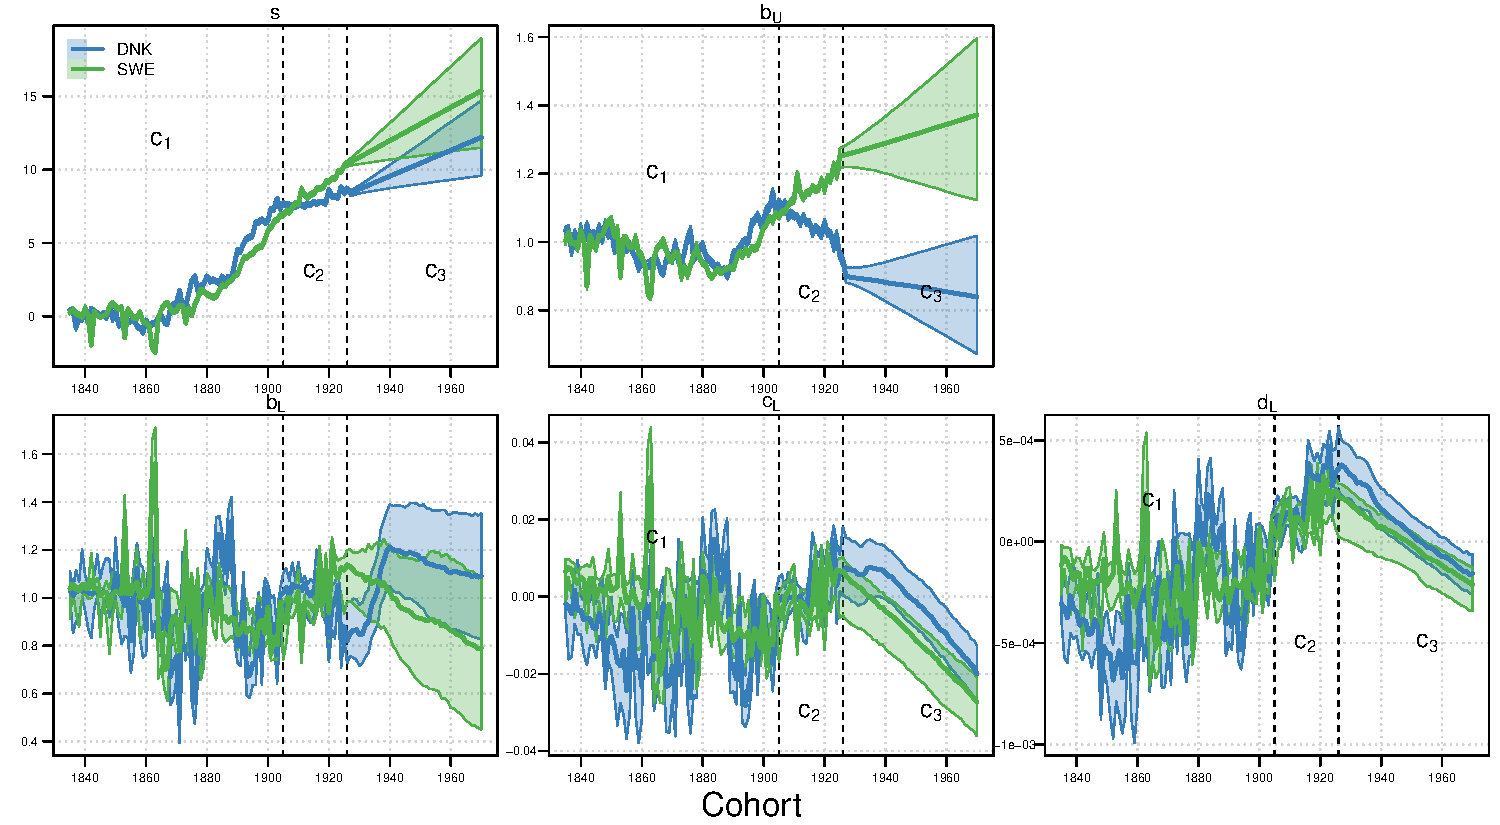
\includegraphics[scale=0.92]{./Figures/FA1.pdf} 
			\caption{Estimated and forecast C-STAD parameters for adult females in Sweden and Denmark for the cohorts 1835--1970. \\ \small \textit{Source}: authors' elaborations on data from the \cite{HMD}.\label{Fig:CSTADparams}}    
		\end{center}
	\end{figure}
\end{landscape}
 
\begin{landscape}
	\begin{figure}[h!]
		\begin{center}
			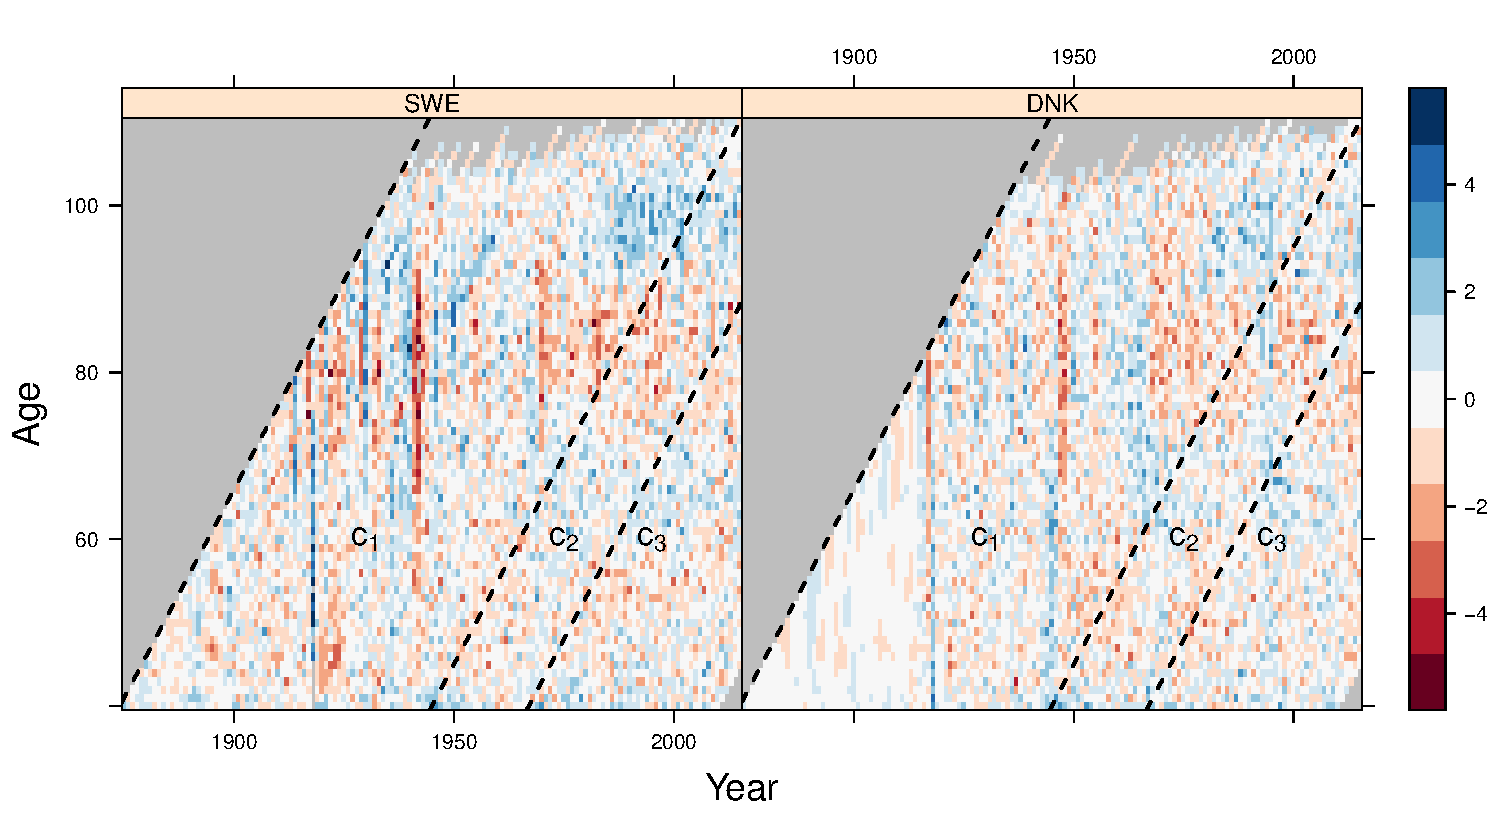
\includegraphics[scale=0.92]{./Figures/FA2.pdf} 
			\caption{Poisson deviance residuals of the C-STAD model for adult females in Sweden and Denmark for the cohorts 1835--1970.\\ \small \textit{Source}: authors' elaborations on data from the \cite{HMD}.\label{Fig:CSTADresid}}    
		\end{center}
	\end{figure}
\end{landscape}


 
\end{document} 